\begin{frame}[fragile]{Merging (1): Branching}
  \begin{itemize}
    \item we have already learned what branches are
    \item we saw how to create them manually
    \item they are intended to be created with
    
  \end{itemize}

\begin{lstlisting}[style=ShellCmd]
$ git branch testing
\end{lstlisting}
  \begin{itemize}
    \item the HEAD of the branch is just pointed to the last commit
    \item ``master'' branch = default name when running ``git init''
  \end{itemize}
  
  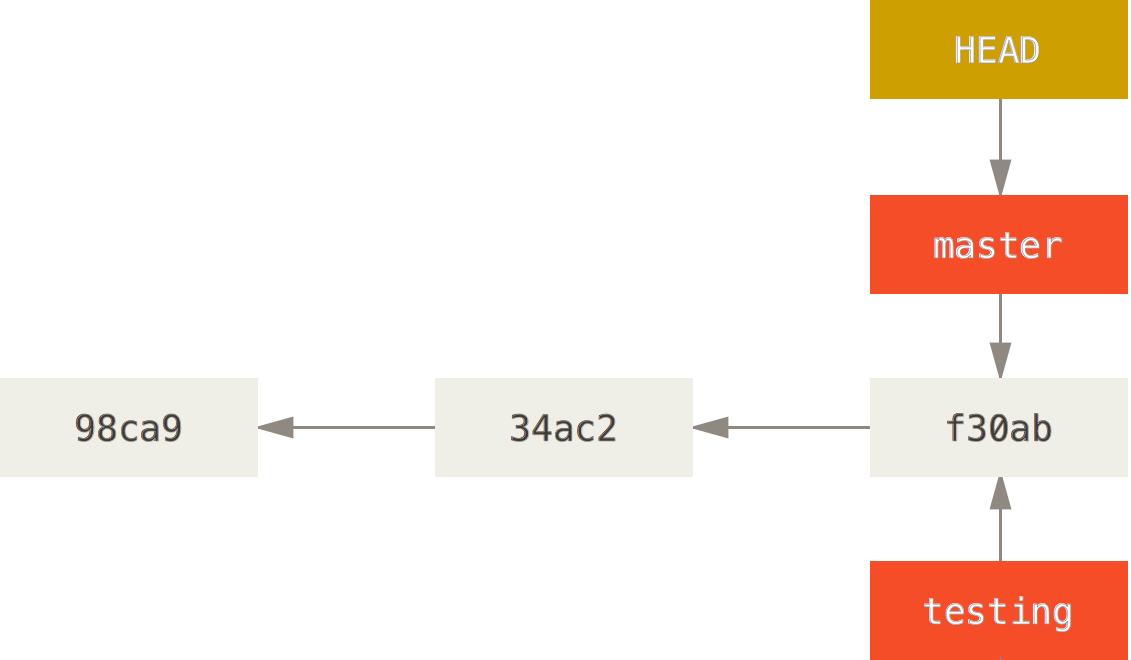
\includegraphics[width=0.50\textwidth]{imgs/head_master}
\end{frame}
\begin{frame}[fragile]{Merging (2): Branching (continued)}
  \begin{itemize}
    \item we can also switch the HEAD and update the working directory with
  \end{itemize}

\begin{lstlisting}[style=ShellCmd]
$ git checkout testing
\end{lstlisting}
  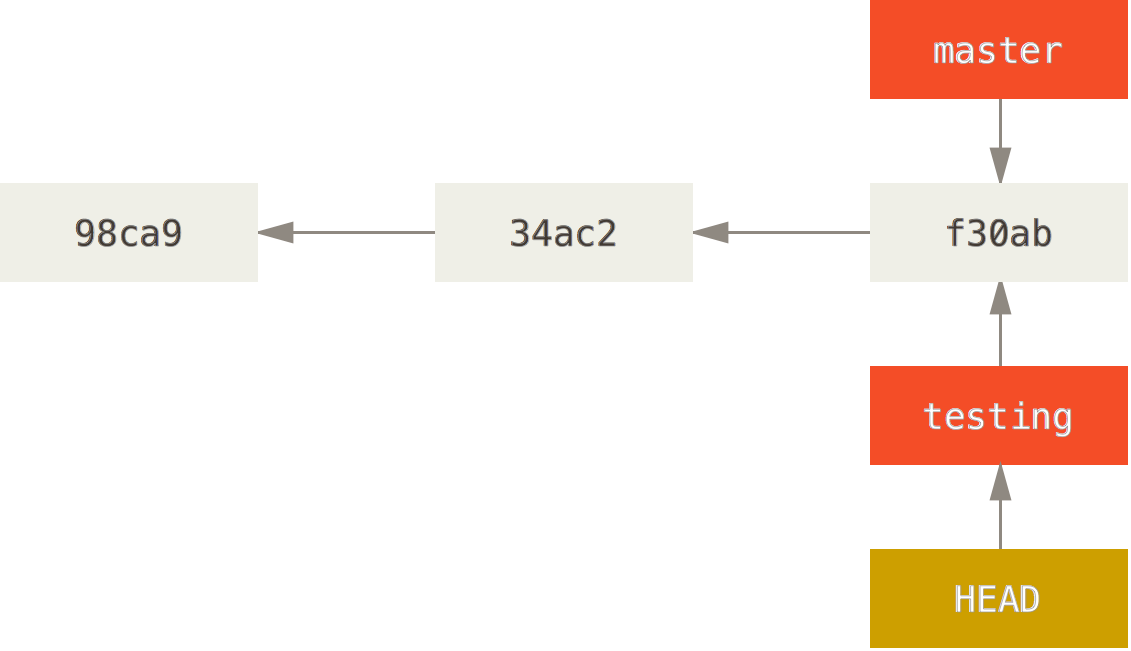
\includegraphics[width=0.50\textwidth]{imgs/head_testing}
\end{frame}

\begin{frame}[fragile]{Merging (3): Merging}
  \begin{itemize}
    \item How to bring branches back together?
    \begin{itemize}
      \item Merging or Rebasing
    \end{itemize}
    \item Merging
    \begin{itemize}
      \item via special ``merge commits'' with more than one parent
      \item they merge changes together using different strategies
    \end{itemize}
    \item Rebase
    \begin{itemize}
      \item rewrite (change history) of all commits since the branching point
      \item ensure both versions are preserved
    \end{itemize}
  \end{itemize}
\end{frame}

\begin{frame}[fragile]{Merging (4): How to merge}
  \begin{itemize}
    
    \item fast-forward-merge = merging two HEADs at two different times
    \begin{itemize}
      \item no conflicts, one just has more commits than the other
      \item simply move the merged HEAD to the newest commit
    \end{itemize}
    
    \item ``Recursive'' merge strategy
    \begin{itemize}
      \item default strategy for non-fast-forward merges
      \item if the same line was modified in conflicting ways there will be merge conflicts
    \end{itemize}
    
    \item Other strategies (we do not go into details)
    \begin{itemize}
      \item ours (take ``our'' version for everything)
      \item theirs (take ``their'' version for everything)
      \item octopus (merge more than 2 HEADs)
      \item subtree
      \item \dots
    \end{itemize}
    
    \item Merge conflicts can occur
    \item Git merges would fill a talk on their own
  \end{itemize}
\end{frame}

\begin{frame}[fragile]{Merging (5): Remotes}
  \begin{itemize}
    
    \item remotes = remote branches
    \begin{itemize}
      \item we can retrieve commits from them
      \item we can push commits to them
    \end{itemize}
    
    \item each branch can have an ``upstream'' branch
    \begin{itemize}
      \item they are called remote-tracking branches
      \item they track the state of the remote
      \item of the form remote/branch
      \item ``origin'' is just the default name for the remote
    \end{itemize}
    
    \item you can fetch commits from a remote branch
    \begin{itemize}
      \item ``git fetch REMOTE BRANCH''
      \item this will update the remote reference , create ``FETCH\_HEAD'' and pull all the commit data
      \item afterwards it can be merged into the current branch
      \item ``git merge FETCH\_HEAD''
    \end{itemize}
  \end{itemize}
\end{frame}

\begin{frame}[fragile]{Merging (6): Remotes continued}
  \begin{itemize}
    
    \item ``git pull'' does this in one go
    \begin{itemize}
      \item does some more magic (for example looking up tracked remote)
      \item make sure everything is checked out into the working directory
      \item sometimes it can be simpler to use ``git fetch'' and then ``git merge''
    \end{itemize}
    
    \item we also want to push content to the remote
    \begin{itemize}
      \item update the server with the changes we made
      \item we can use ``git push REMOTE BRANCH''
      \item each branch can be pushed individually or kept local only
      \item only accepts fast-forward pushes
      \item can be forced with a ``--force'' argument
    \end{itemize}
    
    \item other remote operations
    \begin{itemize}
      \item setting the tracking branch (``git branch -u REMOTE/BRANCH'')
      \item deleting a branch from the remote (``git push REMOTE --delete BRANCH'')
    \end{itemize}
  \end{itemize}
\end{frame}